\chapter{Fundamentação Teórica}\label{cap:CnptDsng}

\section*{Processamento de Áudio}\label{sec:esc_freq}
As gravações de áudio se dão por meio de microfones e captadores de áudio, os quais realizam a conversão por meio de um transdutor, o qual converte a variação da pressão acústica em uma variação de tensão elétrica correspondente. Este sinal é convertido em pequenas amostras individuais espaçadas no tempo de maneira regular, constituindo a aproximação da forma de onda original.

Este processo é conhecido como conversão analógico-digital. O número de amostras retiradas da onda original no período de um segundo, é chamada frequência de amostragem, e quanto mais elevado o seu valor, mais fiel será a representação do sinal no domínio digital. De acordo com o teorema de Nyquist, o limite mínimo para a frequência de amostragem de qualquer sinal é o dobro da sua frequência original. A representação do sinal de áudio no domínio digital é apresentada como uma sequência de palavras onde o número de bits determina a resolução em amplitude do sinal.

No processo de reprodução de áudio, acontece o inverso da situação original, onde o sinal digital é enviado a um conversor digital-analógico, responsável pela reconstrução do sinal para que ele possa ser reproduzido em alto-falantes, caixas de som, ou qualquer aparelho que possa reproduzir sinais de áudio.

Dentro do domínio digital, o sinal de áudio pode ser tratado utilizando todas as técnicas de processamento, tais como as FFTs, DFTs filtros digitais, técnicas de janelamento e filtros digitais. Sendo assim, torna-se extremamente interessante e necessário realizar diversos tratamentos nestes sinais no domínio digital para reduzir as interferências externas, ruídos e desafinação, mantendo assim uma afinação constante em uma música. 

Uma das principais técnicas utilizadas para correção de afinação é a de pitch-shift, a qual consiste na mudança do tom de um sinal de áudio sem modificar o tamanho dele. A diferença de um deslocamento em frequência para o pitch-shift é justamente o fato de que num deslocamento em frequência, existe um deslocamento do espectro do som, enquanto um phase-shift dilata ou comprime o espectro de som.. O Pashe-Vocoder é uma técnica de pitch-shift muito utilizada por produtores musicais.[2][3] 

\begin{figure}[h]
	\centering
	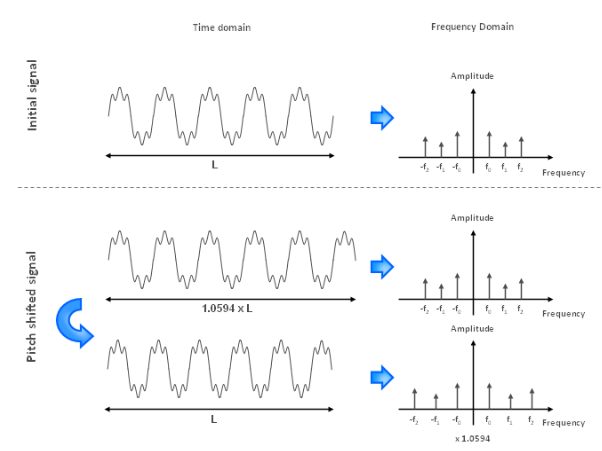
\includegraphics[width=.6\textwidth]{Pitch_Shift.png}
	\label{fig:Pitch_Shif}
	\caption{Demonstração da técnica de Pitch Shift para sinais de guitarra}
	%\source{Própria}
\end{figure}
\newpage

\section*{STFT (Short Time Fourier Transform)}\label{sec:est_obs}
Uma das técnicas mais utilizadas em processamento digital de sinais é a Transformada Discreta de Fourier (DFT), a qual é uma variação da Transformada de Fourier para sinais discretos. A transformada de Fourier define a redução de uma função periódica a um somatório de senos e cossenos. Este procedimento matemático gera uma representação de um sinal originalmente no domínio do tempo, em uma representação no domínio da frequência.[4]

\begin{figure}[h]
	\centering
	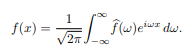
\includegraphics[width=.3\textwidth]{Fourier.png}
	\label{fig:Fourier}
	\caption{Transformada de Fourier para sinais contínuos}
	%\source{Própria}
\end{figure}

\begin{figure}[h]
	\centering
	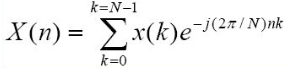
\includegraphics[width=.5\textwidth]{DFT.png}
	\label{fig:DFT}
	\caption{Transformada Discreta de Fourier}
	%\source{Própria}
\end{figure}

As transformadas de Fourier se aplicam somente a sinais de funções estacionárias, onde o espectro de frequência é fixo e não variam com o tempo.

Os sinais de áudio gerados pela voz humana se encontram dentro do espectro de frequências entre 50 a 3400 Hz, e a sua principal característica é a de que a sua frequência não é constante no tempo, o que dá ao sinal da voz humana a característica da não-ergodicidade (seu sinal não mantém as propriedades estatísticas ao longo do tempo), sendo assim, a utilização da STFT (Short Time Fourier Transform) se torna bastante eficaz em sinais dessa natureza.

A STFT é um algoritmo desenvolvido com base na transformada discreta de Fourier, diferenciando-se pela inclusão de uma função de janelamento w(t). Sua principal aplicação é para funções cujo o espectro de frequência varia com o tempo.[4]

\begin{figure}[h]
	\centering
	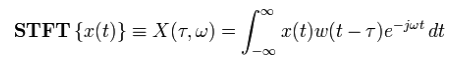
\includegraphics[width=.6\textwidth]{STFT.png}
	\label{fig:STFT}
	\caption{Transformada de Fourier de Tempo Curto}
	%\source{Própria}
\end{figure}

\begin{figure}[h]
	\centering
	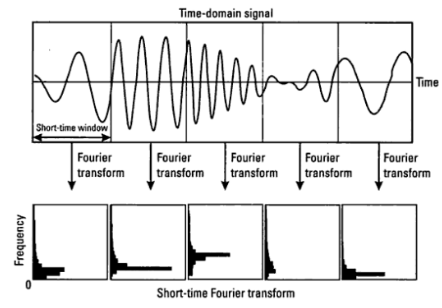
\includegraphics[width=.7\textwidth]{STFT_GRAPHICS.png}
	\label{fig:STFT_GRAPHICS}
	\caption{Transformada de Fourier de Tempo Curto sendo aplicada em diversas frequências de um mesmo sinal}
	%\source{Própria}
\end{figure}
 
O principal propósito da utilização de uma STFT é separar o sinal em pequenos intervalos que possam ser tratados individualmente, obtidos através da janela que está inserida na transformada. Desta maneira a modificação de frequência se dá de forma independente, sem a alteração de tempo e vice versa. 

\section*{Funções de Janelamento}
Para aplicações que consistem na amostragem de sinais, a amostragem, por ser finita, resulta em uma forma de onda truncada com características diferentes do sinal original, consequentemente a influência do vazamento espectral torna-se maior para uma situação como esta, gerando uma perda de informação do sinal original. 
Para reduzir os efeitos das imperfeições de amostragem, melhorando a qualidade da reconstrução do sinal é a aplicação de uma função de janelamento.[5]

\begin{figure}[h]
	\centering
	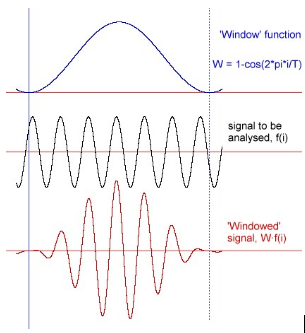
\includegraphics[width=.7\textwidth]{Janelamento.png}
	\label{fig:Janelamento}
	\caption{Efeitos da função de janelamento em um sinal no espectro de frequência}
	%\source{Própria}
\end{figure}
 \newpage

A utilização de uma função de janelamento permite uma definição do período de observação do sinal, redução dos efeitos do vazamento espectral e a separação do sinal de pequena amplitude com frequências muito próximas. A aplicação de uma função de janelamento no tempo, consiste na multiplicação da função original pela função, o que equivale a uma convolução no domínio da frequência.
Existem diversas funções de janelamento, as quais possuem diferentes características e aplicações dependendo principalmente dos parâmetros desejados do sinal original.

\begin{itemize}
	\item Retangular
	\item Hanning
	\item Hamming
	\item Blackman
	\item Kaiser-Bessel
\end{itemize}
 
\section*{Janela Hanning}

Dentre as funções de janelamento existentes, a função Hanning é a mais comumente utilizada na produção musical. O formato desta janela é similar ao de meio ciclo de uma onda cossenoidal. Suas características de baixo vazamento espectral e  formato de onda bem similar ao formato cossenóide,. Torna-se recomendável utilizar portanto a janela para análises de sinais com transientes maiores que de duração da própria janela.

\begin{figure}[h]
	\centering
	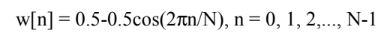
\includegraphics[width=.7\textwidth]{Janela_Hanning.png}
	\label{fig:Janela Hanning}
	\caption{Função da janela Hanning}
	%\source{Própria}
\end{figure}

\begin{figure}[h]
	\centering
	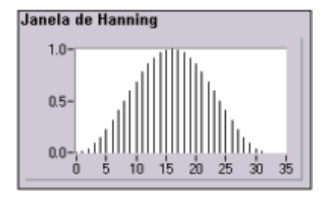
\includegraphics[width=.5\textwidth]{Grafico_Hanning.png}
	\label{fig:Gráfico Hanning}
	\caption{Gráfico da janela Hanning}
	%\source{Própria}
\end{figure}

\newpage

\chapter{Metodologia}
\section*{Funcionamento da solução}
Utilizando o software MATLAB, uma solução computacional foi desenvolvida para realizar o procedimento de regulagem de tom. 

O funcionamento do algoritmo se dá primeiramente com a captação do áudio por meio dos microfones. Logo em seguida é aplicada a STFT para detecção dos espectros de frequência presentes no sinal de áudio. 

A detecção da frequência mais próxima se dá para que o Pitch-Shift seja realizado corretamente e logo em seguida o sinal seja reconstruído.

Para a reprodução do sinal é realizada a transformada inversa de Fourier para que o sinal seja colocado no tempo.

\begin{figure}[h]
	\centering
	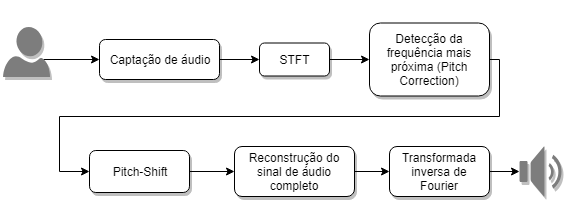
\includegraphics[width=.9\textwidth]{Fluxograma_Solucao.png}
	\label{fig:Fluxograma_Solucao}
	\caption{Fluxograma de Funcionamento do algoritmo desenvolvido}
	%\source{Própria}
\end{figure}

\section*{Funções Utilizadas}
\subsection*{gravaAudio}
Função responsável por gravar o áudio à ser utilizado para afinação. Recebendo como parâmetros de entrada a frequência de amostragem fs e a duração do áudio. Retorna o aúdio gravado.

\subsection*{istft}
Função responsável por realizar a transformada inversa da stft. Recebe como parâmetros de entrada o conjugado do sinal a ser convertido, o número de amostras da stft, a quantidades de bins N da janela, e quantidade de bins que não sofrerão overlap. Retorna o sinal reconstruído

\subsection*{spectrogram}
Função responsável por fazer a stft, recebendo como argumentos  o sinal, a janela a ser utilizada, quantidade de amostras da FFT, quantidade de amostras que não sofrerão overlap e frequência de amostragem. Retornando um vetor contendo o sinal transformado, um vetor de frequências F, um vetor de tempo T e um vetor de densidade espectral de potência.

\subsection*{conj}
Retorna o complexo conjugado dos elementos contidos no argumento.


\subsection*{mostraEspectograma}
Mostra o spectrograma do sinal S, recebendo o vetor de frequência F e o vetor de tempo T.

\subsection*{tabela Do Maior}
Retorna um vetor contendo todas as frequências da escala de Dó Maior.]

\subsection*{compareToPitches}
A função recebe um tom e a tabela contendo a escola de tons, retornando o tom mais próximo da escala. 

\subsection*{pitchCorrector}
Função responsável por corrigir a stft, colocando os tons na escala fornecida. Recebe como entrada a STFT, seu espaço em frequência, o vetor de densidade espectral de potência P e tabela com a escala de tons. Retoranndo a stft corrigida.

\subsection*{sound}
Toca o sinal de som fornecido, recebendo o som e a frequência de amostragem.

